\documentclass{article}
\usepackage{float}
\usepackage{amsmath}
\usepackage{hyperref}
\usepackage{xcolor}
\usepackage{algpseudocode}
\usepackage{algorithm}
\usepackage{amssymb}
\usepackage{caption}
\usepackage{subcaption}
\usepackage[margin=1in, top=0.5in]{geometry} 
\usepackage{graphicx} % Required for inserting images

\title{Jane Street Puzzle June 2026}
\author{Andrew Ely}
\date{}

\begin{document}
\maketitle


\begin{center}
\section*{Regional Artwork}
\end{center}

\begin{figure}[H]
    \centering
    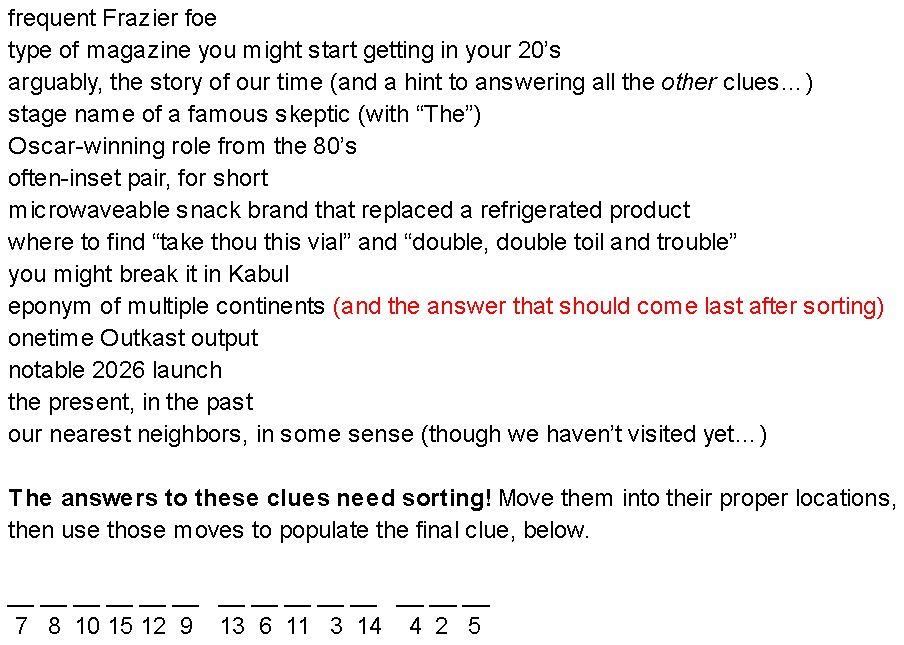
\includegraphics[width=1\linewidth]{img.jpg}
\end{figure}


\section*{Understanding The Problem}

This months puzzle does not have very clear instructions. We must do some deciphering and inferring to understand and solve the puzzle. Some first observations we can make is that we have 14 clues, and 14 blank spaces. Some of the clues have additional hints, and there is some context provided for the final solution, suggesting we need to sort the clues. 

So, the puzzle seems to consist of answering each clue, then preforming some type of sorting. The third clue says it will be a hint to answering all the other clues, so finding an answer for that one should provide more direction. 

As a strategy, we can start brainstorming potential answers to each clue by google searching. After coming up with potential answers for each clue, we can look for overlap between the answers we are more confident about and the third clue. Then, we can continue refining our answers to all the other clues by refining our lists based on the hint given by the third clue.

\section*{Solving the problem}

\subsection*{Initial Searches}

Relying on just google searches for now, we can google search each of the clues and record potential answers based on top results and some short exploration, like Wikipedia pages or other top result pages. Doing this, we come up with the following,

\quad

\textbf{clue 1: } frequent Frazier foe

\quad\textbf{potential answers:} Ali, Muhammad Ali

\quad

\textbf{clue 2: } type of magazine you might start getting in your 20's

\quad\textbf{potential answers:} New York Times, People,  academic journals, 

\quad

\textbf{clue 3: } arguably, the story of our time 

\quad\textbf{potential answers:} Robert Atkinson, Christopher Hitchens, "Arguably"

\quad

\textbf{clue 4: } stage name of a famous skeptic (with "The")

\quad\textbf{potential answers:} The Amazing Randi, Amazing Randi

\quad

\textbf{clue 5: } Oscar-winning role from the 80's

\quad\textbf{potential answers:} Dustin Hoffman, Robert De Niro, Henry Fonda, Ben Kingsley, Robert Duvall, F. Murray Abraham, William Hurt, Paul Newman, Michael Douglas

\quad

\textbf{clue 6: } often-inset pair, for short

\quad\textbf{potential answers:} Alaska/Hawaii

\quad

\textbf{clue 7: } microwaveable snack brand that replaced a refrigerated product

\quad\textbf{potential answers:} Hotpockets, Micro Magic

\quad

\textbf{clue 8: } where to find "take thou this vial" and "double, double toil and trouble"

\quad\textbf{potential answers:} Shakespeare, William Shakespeare

\quad

\textbf{clue 9: } you might break it in Kabul

\quad\textbf{potential answers:} Breakfast, Bread, Pul, Afghani

\quad

\textbf{clue 10: } eponym of multiple continents

\quad\textbf{potential answers:} Pangaea, Amerigo, Amerigo Vespucci

\quad

\textbf{clue 11: } onetime Outkast output

\quad\textbf{potential answers:} In Due Time, Da Art of Storytellin', Aquemeni, ATLiens 

\quad

\textbf{clue 12: } notable 2026 launch

\quad\textbf{potential answers:} Artemis II

\quad

\textbf{clue 13: } the present, in the past

\quad\textbf{potential answers:} The Future

\quad

\textbf{clue 14: } our nearest neighbors, in some sense (though we haven't visited yet...) 

\quad\textbf{potential answers:} Mars, Venus, Proxima Centauri, Alpha Centauri

\quad 

After initial brainstorming, we can realize some answers are much more likely correct than others. We can be confident of some clues like 1, 4, 6, and 12, while clues like 2, 3, 5, and others do not seem to have well fitting answers yet. Taking the most confident answers: Ali (Muhammed Ali), Amazing Randi (The Amazing Randi), Alaska/Hawaii, Atermis II, we can look for a pattern between these answers.

The biggest realization for solving the puzzle is that all of these answers start with the letter ``A" and end with the letter ``I". Then, the answer to clue 3 can be AI (Artificial Intelligence), which is definitely fitting as `the story of our time'.

Now, with our new constraint that clues must start with the letter ``A" and end with letter ``I", we can refine our list of potential answers for clues like 9, 10, 11, and 14. We still need answers for clues 2, 5, 7, 8, and 13. 

Also, the instructions at the end of the puzzle tells us the answers need sorting. We also have the additional hint that clue 10's answer should come last after sorting, which is the clue that is 15 characters long. There are 14 blanks, labeled 2 through 15. If we start with clue 3 being "AI", 2 letters long, then each clue's answer can be a unique length. Making adjustments like this, we result in the following refined search.

\subsection*{Refined Search}

\begin{tabular}{ c c c }
 \textbf{Clue} & \textbf{Answer} & \textbf{Num Characters} \\ 
 1 & Ali &  3\\  
 2 & ??? &  ???\\
 3 & AI &  2\\
 4 & Amazing Randi &  12\\
 5 & ??? &  ???\\
 6 & AL,HI &  4\\
 7 & ??? &  ???\\
 8 & ??? &  ???\\
 9 & Afghani &  7\\
 10 & Amerigo Vespucci &  15\\
 11 & Aquemini &  8\\
 12 & Artemis II &  9\\
 13 & ??? &  ???\\
 14 & Alpha Centauri & 13   
\end{tabular}

\quad

\quad

So, to follow with our hypothesis, we need words that start with the letter A, end with the letter I, and are 5,6,10,11, and 14 letters long, and fit the remaining clues. Using these constraints, we can solve the more obscure remaining clues:

\quad

\textbf{clue 2: } type of magazine you might start getting in your 20's

\quad\textbf{answer:} Alumni

\quad\textbf{explanation:} An alumni magazine is a type of magazine you can get about your college after you graduate.

\quad

\textbf{clue 5: } Oscar-winning role from the 80's

\quad\textbf{answer:} Antonio Salieri

\quad\textbf{explanation:} The movie ``Amadeus" (1984) won 8 awards from the Oscars, including the lead actor F Murry Abraham who played Antonio Salieri, an Italian composer. 

\quad


\textbf{clue 7: } microwaveable snack brand that replaced a refrigerated product

\quad\textbf{answer:} Act II

\quad\textbf{explanation:} This microwavable popcorn brand replaced the brand Act I, which had to be refrigerated because it contained real butter, while Act II does not.

\quad

\textbf{clue 8: } Where to find ``take thou this vial" and ``double, double toil and trouble"

\quad\textbf{answer:} Act IV, Scene I

\quad\textbf{explanation:} Both of these Shakespeare quotes can be found in Romeo and Juliet, and Macbeth, both in Act four Scene in either play. 

\quad

\textbf{clue 13: } the present, in the past

\quad\textbf{answer:} Anno Domini 

\quad\textbf{explanation:} This is what A.D stands for when using (AD) and (BC) to refer to time periods.

\quad

All of these answers fit to give unique lengths of characters between 2 and 15. Now, we have to sort and determine what letter corresponds to each clue. The way to sort that works it to arrange all the answers by length of answer from shortest to longest. Then, we count the number of spaces we had to shift that answer and take the character in the answer at the numbers position. In other words, we take the absolute value of the original clue position (1 to 14) minus its new position, plus one. Then we take the character at that position in the answer, as follows:

\begin{tabular}{ c c c c c }
 \textbf{Clue} & \textbf{Answer} & \textbf{Num Characters} & \textbf{Shift} & \textbf{Letter} \\ 
 1 & Ali &  3 &  1 &  A\\  
 2 & Alumni &  6 &  3 &  U\\
 3 & AI &  2 & 2 &  I\\
 4 & Amazing Randi &  12 &  7 &  G\\
 5 & Antonio Salieri &  14 &  8 &  S\\
 6 & AL,HI &  4 &  3 &  H\\
 7 & Act II &  5 &  3 &  T\\
 8 & Act IV, Scene I &  11 &  2 &  C\\
 9 & Afghani &  7 &  3 &  G\\
 10 & Amerigo Vespucci &  15 &  4 &  R\\
 11 & Aquemini &  8 &  4 &  E\\
 12 & Artemis II &  9 &  4 &  E\\
 13 & Anno Domini  &  10 &  4 &  O\\
 14 & Alpha Centauri & 13 &  2 &  L  
\end{tabular}

\quad

And populating the final clue by taking the number under the blanks clue number, and that clue numbers corresponding Letter from the table above, we get the final clue:

\quad

George Lucas Hit 

\quad

Following the same constraints as the rest of the puzzle, and as hinted at by the title of the puzzle ``Regional Artwork", the final answer is:

\quad

\textbf{American Graffiti}

\end{document}
